\subsection{Modelling the airflow}
\large \emph{\textbf{Mohamed Rekik}}

In the field of aerodynamics, modeling the airflow around an object such as an airplane wing is crucial to understanding its performance. In this particular case, the airflow around a previously interpolated wing will be modeled using a laminar flow assumption. Laminar flow means that the airflow can be divided into two parts, and each air molecule moves along curves that do not intersect. This is an important assumption because it simplifies the modeling process and allows for more accurate predictions.

To model the airflow, the minimum and maximum height of the airflow were first determined to be $h_{min}^{m}$ and $h_{max}^{m}$, respectively. The airflow is assumed to be disturbed by the wing in a vertical interval of $[[3h_{min}; 3h_{max}]]$, while it is rectilinear elsewhere. This assumption is necessary to accurately capture the effect of the wing on the airflow.

The next step is to model the curve $y$ for either the extrados or the intrados. The curve $y$ represents the shape of the upper or lower surface of the wing. This is done using the equation given in (\ref{eq:equation_part3.1}), where $f(x)$ is the function that interpolates the points of the wing, and $\lambda$ is a parameter that varies between 0 and 1. The value of $\lambda$ determines the shape of the curve, with a value of 0 resulting in the original shape of the wing and a value of 1 resulting in a straight line at a height of $h_{max}\times 3$. By varying $\lambda$ between 0 and 1, the shape of the wing can be smoothly transitioned from its original shape to a straight line.
\begin{equation}
  \label{eq:equation_part3.1}
  y = f_{\lambda}(x) = (1 - \lambda)f(x) + \lambda \times h_{max} \times 3 \quad \forall \lambda \in [0,1] 
\end{equation}

To confirm the laminar nature of the airflow, several measurements are taken. These include the extrados $x/y$ $(ex, ey)$, the intrados $x/y$ $(ix, iy)$, the function that interpolates the points of the upper part of the wing (fint\_upp), and the function that interpolates the points of the lower part of the wing (fint\_low). A figure is obtained (see Figure \ref{fig:laminar}), which confirms the laminar nature of the airflow. The figure shows that the airflow above and below the wing follows a smooth and regular pattern, which is indicative of laminar flow.
\begin{figure}[H]
  \centering
  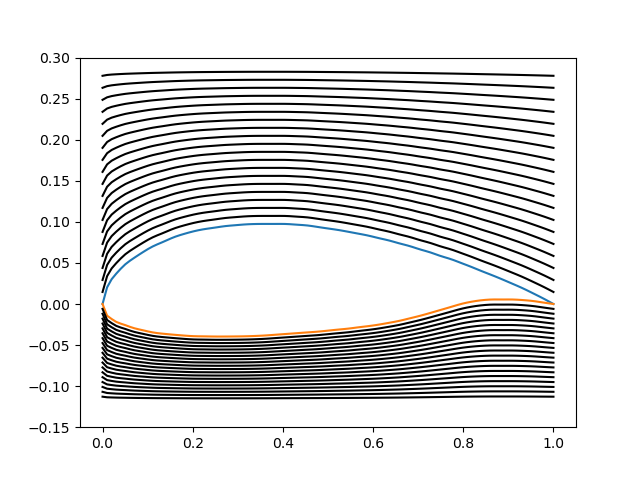
\includegraphics[width=0.45\textwidth]{img/laminar_flow.png}
  \caption{Laminar flow above and below the wing}
  \label{fig:laminar}
\end{figure}

In conclusion, modeling the airflow around a wing is an important step in understanding its performance. By assuming laminar flow and using various measurements, the shape of the airflow can be accurately predicted. This information is crucial for designing and optimizing airplane wings, and can lead to improved performance and efficiency.

\subsection{Pressure map}
\large \emph{\textbf{Mohamed Dyae Chellaf}}

As in the first subsection, we will use functions defined in the previous sections to approach the study of this subsection.
We must plot the function corresponding to the pressure distribution around the wing to have even more information on the aerodynamic profile and thus improve performance and characteristics.\\
We can ultimately come to understand the behavior of the air around the airfoil.\\
Given a laminar airflow, the particles move along independent trajectories.\\
In this sequence, we base ourselves on the distribution of the pressure in the surface of the aerodynamic profile drawn and we save the results.\\
And so does the pressure map obteined shows the informations about the airflow around the airfoil, and shows that the air moves more easily above the wing than below, which leads to a remarkable pressure difference, which in turn creates a lift force that gives the plane the ability to stay aloft?\\
\begin{figure}[h]
  \centering
  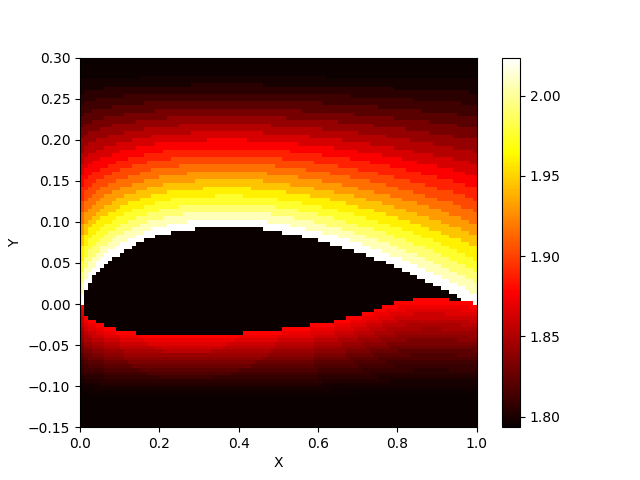
\includegraphics[width=0.45\textwidth]{img/pressure_map.png}
  \caption{Pressure map}
  \label{fig:pressure}
\end{figure}

